% Appendix
\section{Appendix}

\subsection{Additional Figures}

\subsubsection{Variable Metric Bundle Method}

The following plots show the behavior in accuracy and number of steps of the proximal bundle algorithm \ref{sec_nonconv_inex}.1 and different realizations of the variable metric bundle method \ref{sec_variable_metric}.1 when optimizing the Ferrier polynomials \(f_1\) to \(f_5\) in different dimensions and for different noise forms.
The conditions and parameters used for the plots are described in section \ref{sec_num_test_ferr}

The two plots below depict the situation for \(x \in \R^n\) for \(n = 2,3,...,15\).

\begin{figure}[H]
	\begin{subfigure}{0.49\textwidth}
		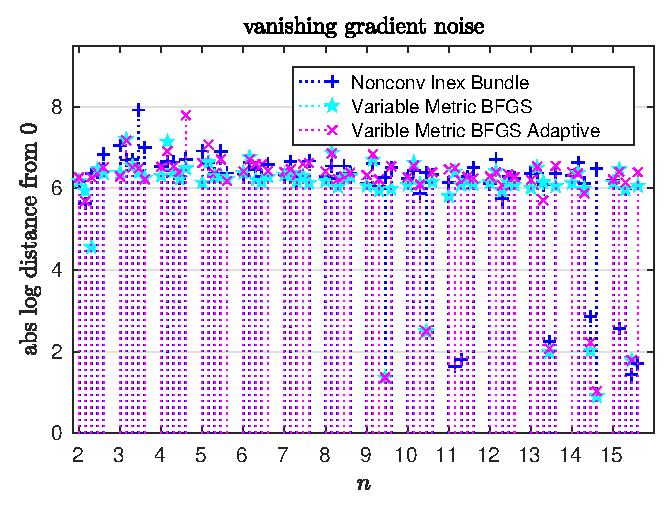
\includegraphics[width=\textwidth]{Pictures/Plots/vanishing_gradient_noise.eps}%
	\end{subfigure}
	\begin{subfigure}{0.49\textwidth}
		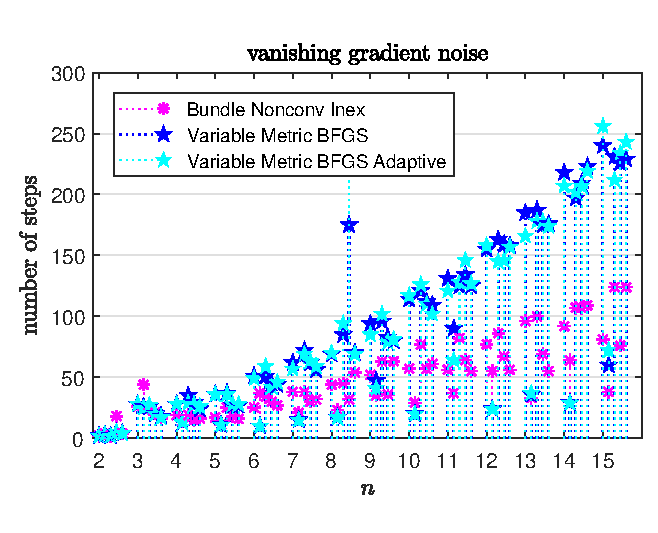
\includegraphics[width=\textwidth]{Pictures/Plots/steps_vanishing_gradient_noise.eps}%
	\end{subfigure}
	\caption{Comparison of accuracy and number of steps for the proximal bundle algorithm and the variable metric bundle algorithm in the case of vanishing gradient noise}%
	\label{fig_van_grad_noise}%
\end{figure}


The following plots show the situation for larger dimensions \(n = 20,25,30,40,50\).


\begin{figure}[H]%
	\begin{subfigure}{0.49\textwidth}
		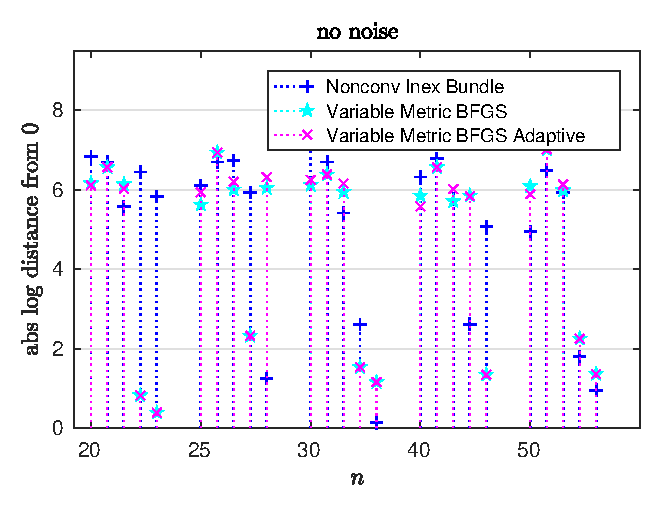
\includegraphics[width=\textwidth]{Pictures/Plots/no_noise_b.eps}%
	\end{subfigure}
	\begin{subfigure}{0.49\textwidth}
		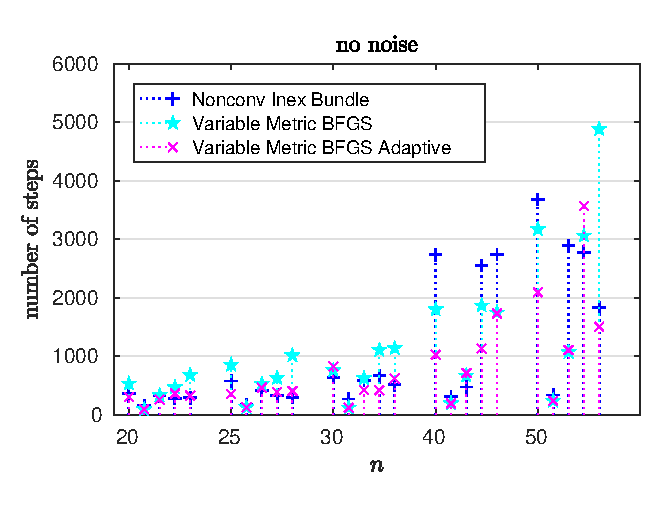
\includegraphics[width=\textwidth]{Pictures/Plots/steps_no_noise_b.eps}%
	\end{subfigure}
	\label{fig_no_noise_large}
	\caption{Comparison of accuracy and number of steps for the proximal bundle algorithm and the variable metric bundle algorithm in the case of no noise}
\end{figure}

\vspace{-1.5em}

\begin{figure}[H]
	\begin{subfigure}{0.49\textwidth}
		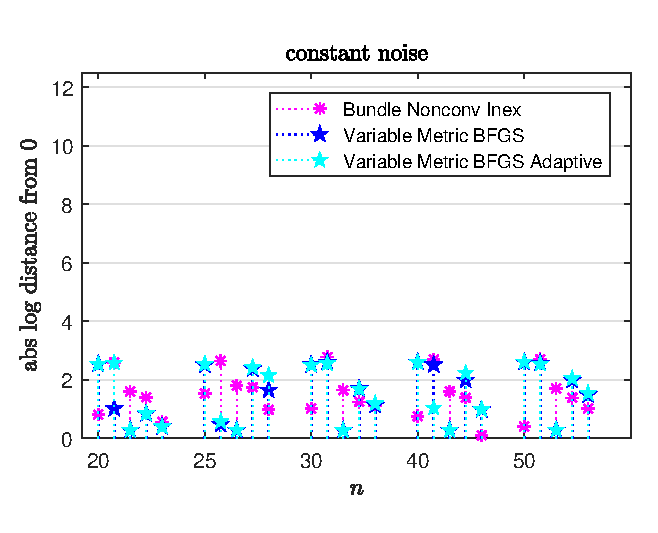
\includegraphics[width=\textwidth]{Pictures/Plots/constant_noise_b.eps}%
	\end{subfigure}
	\begin{subfigure}{0.49\textwidth}
		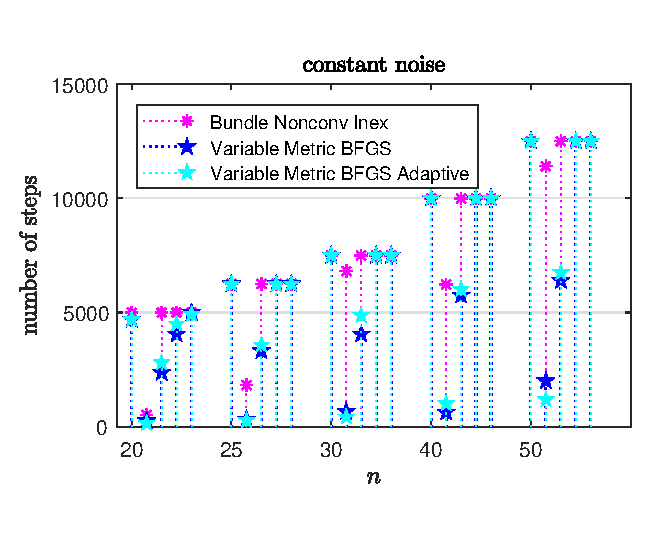
\includegraphics[width=\textwidth]{Pictures/Plots/steps_constant_noise_b.eps}%
	\end{subfigure}
	\vspace{-.5em}
	\caption{Comparison of accuracy and number of steps for the proximal bundle algorithm and the variable metric bundle algorithm in the case of constant noise}%
	\label{fig_const_noise_large}%
\end{figure}

\vspace{-1.5em}

\begin{figure}[H]
	\begin{subfigure}{0.49\textwidth}
		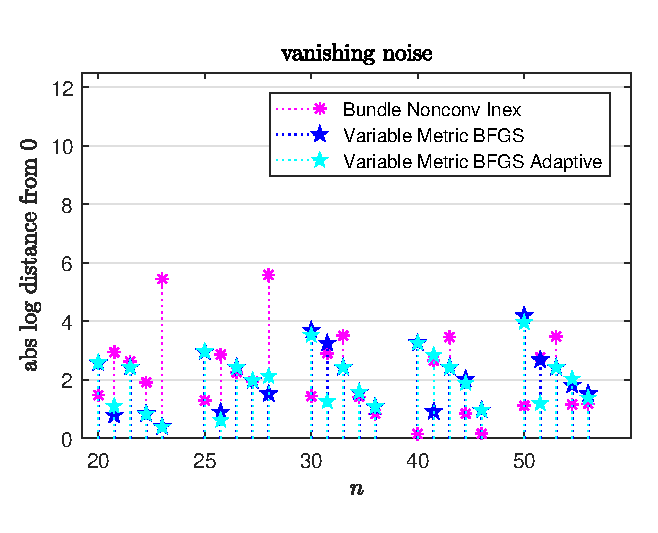
\includegraphics[width=\textwidth]{Pictures/Plots/vanishing_noise_b.eps}%
	\end{subfigure}
	\begin{subfigure}{0.49\textwidth}
		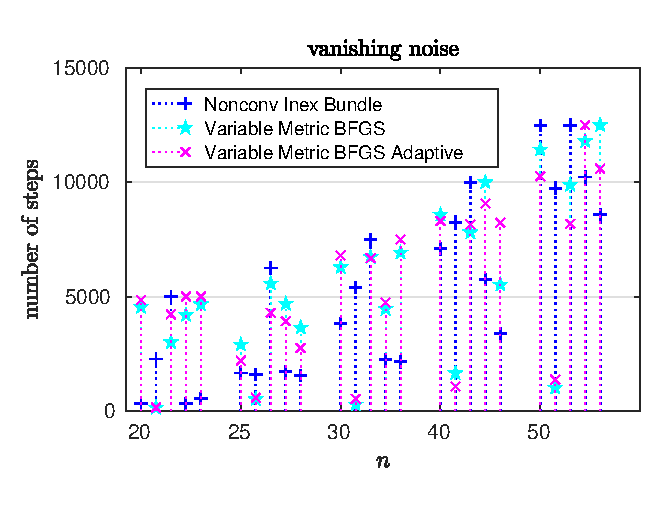
\includegraphics[width=\textwidth]{Pictures/Plots/steps_vanishing_noise_b.eps}%
	\end{subfigure}
	\caption{Comparison of accuracy and number of steps for the proximal bundle algorithm and the variable metric bundle algorithm in the case of vanishing noise}%
	\label{fig_van_noise_large}%
\end{figure}

\vspace{-1.5em}

\begin{figure}[H]
	\begin{subfigure}{0.49\textwidth}
		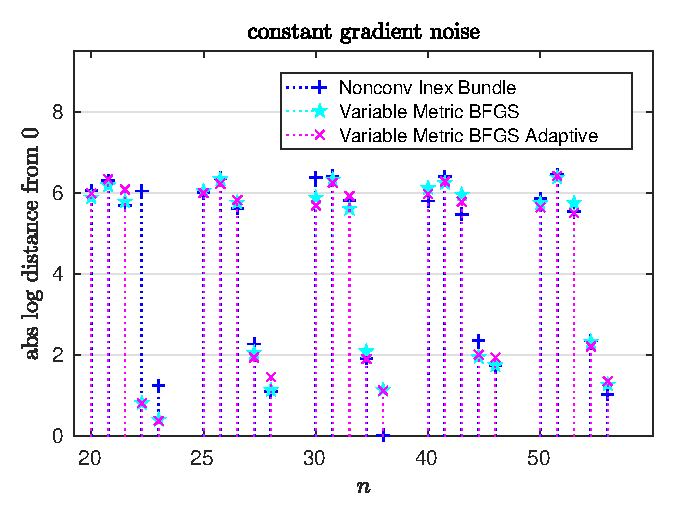
\includegraphics[width=\textwidth]{Pictures/Plots/constant_gradient_noise_b.eps}%
	\end{subfigure}
	\begin{subfigure}{0.49\textwidth}
		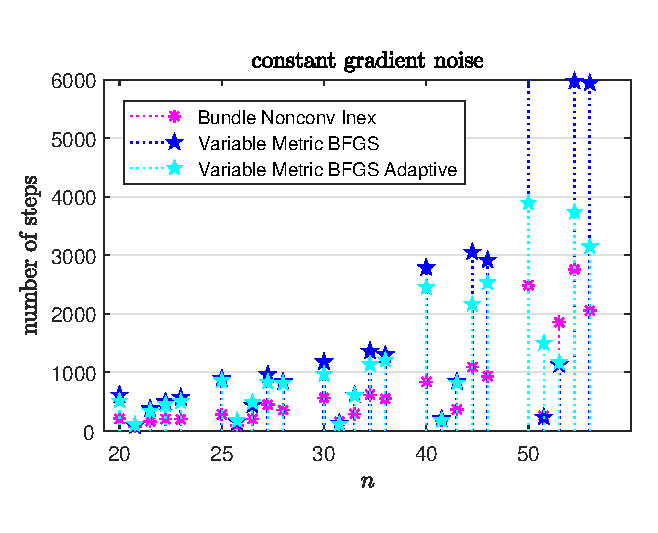
\includegraphics[width=\textwidth]{Pictures/Plots/steps_constant_gradient_noise_b.eps}%
	\end{subfigure}
	\caption{Comparison of accuracy and number of steps for the proximal bundle algorithm and the variable metric bundle algorithm in the case of constant gradient noise}%
	\label{fig_const_grad_noise_large}%
\end{figure}

\vspace{-1.5em}

\begin{figure}[H]
	\begin{subfigure}{0.49\textwidth}
		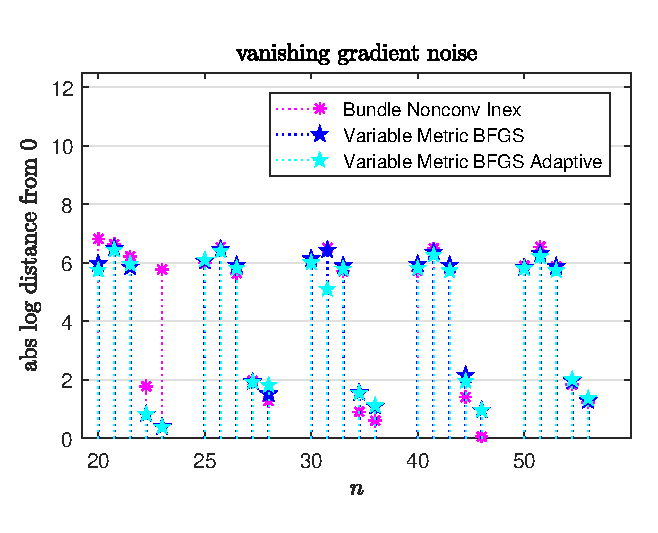
\includegraphics[width=\textwidth]{Pictures/Plots/vanishing_gradient_noise_b.eps}%
	\end{subfigure}
	\begin{subfigure}{0.49\textwidth}
		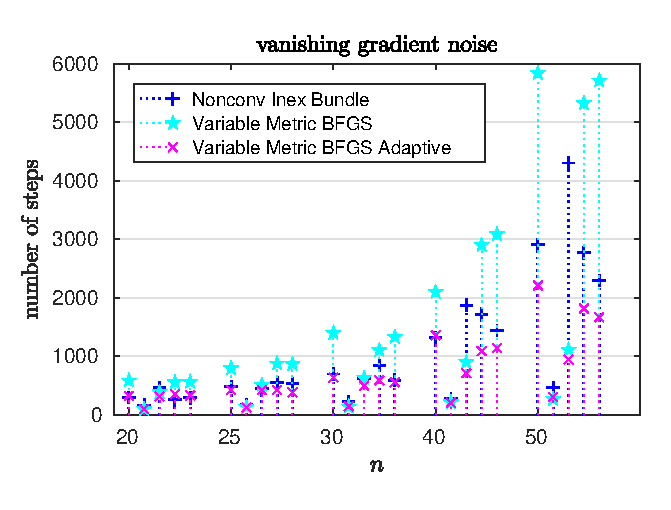
\includegraphics[width=\textwidth]{Pictures/Plots/steps_vanishing_gradient_noise_b.eps}%
	\end{subfigure}
	\caption{Comparison of accuracy and number of steps for the proximal bundle algorithm and the variable metric bundle algorithm in the case of vanishing gradient noise}%
	\label{fig_van_grad_noise_large}%
\end{figure}

Next come the figures that illustrate the difference in behavior for different step size updating parameter \(\kappa_+\) and the performance of the hybrid method. In this method the metric matrix is scaled for boundedness of the eigenvalues and then scaled again by \(1/k\).


\begin{figure}[H]
	\begin{subfigure}{0.49\textwidth}
		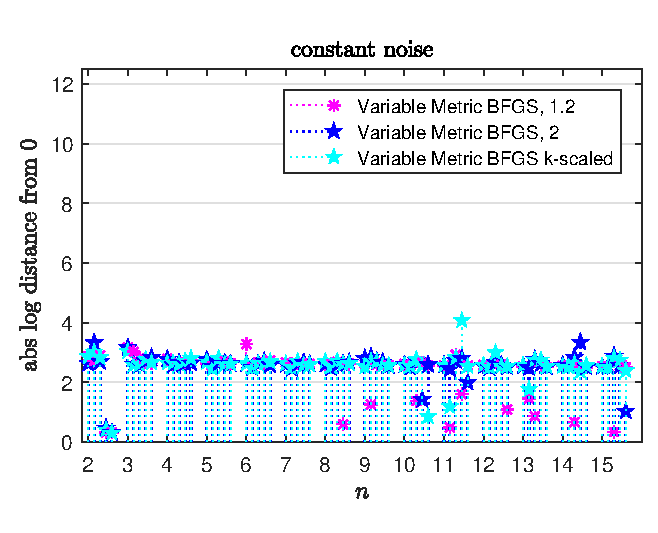
\includegraphics[width=\textwidth]{Pictures/Plots/constant_noise_comp.eps}%
	\end{subfigure}
	\begin{subfigure}{0.49\textwidth}
		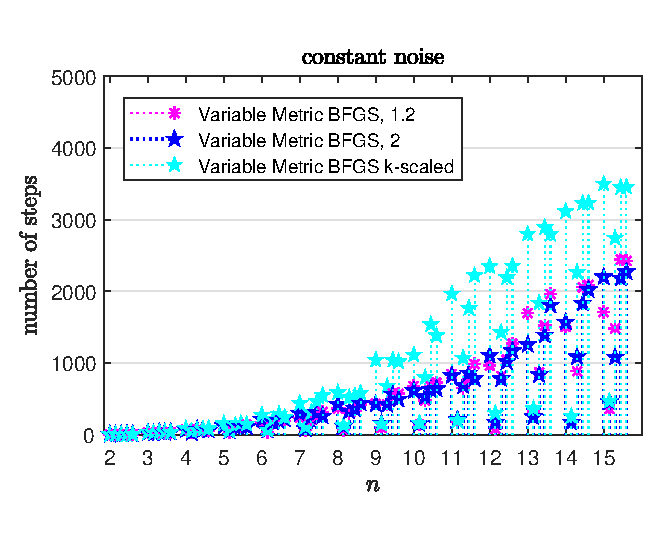
\includegraphics[width=\textwidth]{Pictures/Plots/steps_constant_noise_comp.eps}%
	\end{subfigure}
	\caption{Influence of the step size updating parameter \(\kappa_+ = 1.2\) and \(\kappa_+ =2 \) and performance of the hybrid method for constant noise. The reached accuracy is depicted on the left, the needed number of steps on the right.}%
	\label{fig_const_noise_comp}%
\end{figure}

\vspace{-1.5em}

\begin{figure}[H]
	\begin{subfigure}{0.49\textwidth}
		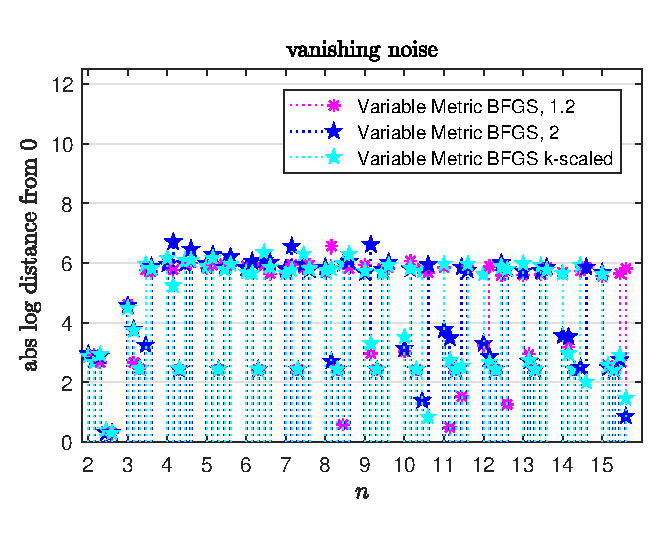
\includegraphics[width=\textwidth]{Pictures/Plots/vanishing_noise_comp.eps}%
	\end{subfigure}
	\begin{subfigure}{0.49\textwidth}
		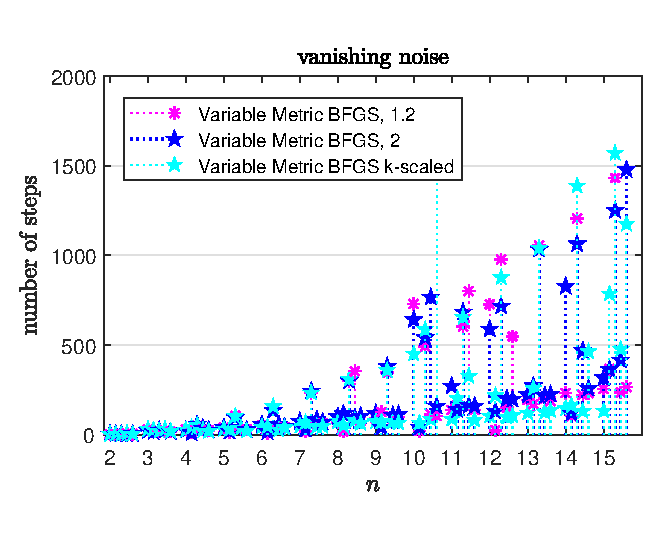
\includegraphics[width=\textwidth]{Pictures/Plots/steps_vanishing_noise_comp.eps}%
	\end{subfigure}
	\caption{Influence of the step size updating parameter \(\kappa_+ = 1.2\) and \(\kappa_+ =2 \) and performance of the hybrid method for vanishing noise.}%
	\label{fig_van_noise_comp}%
\end{figure}

\vspace{-1.5em}

\begin{figure}[H]
	\begin{subfigure}{0.49\textwidth}
		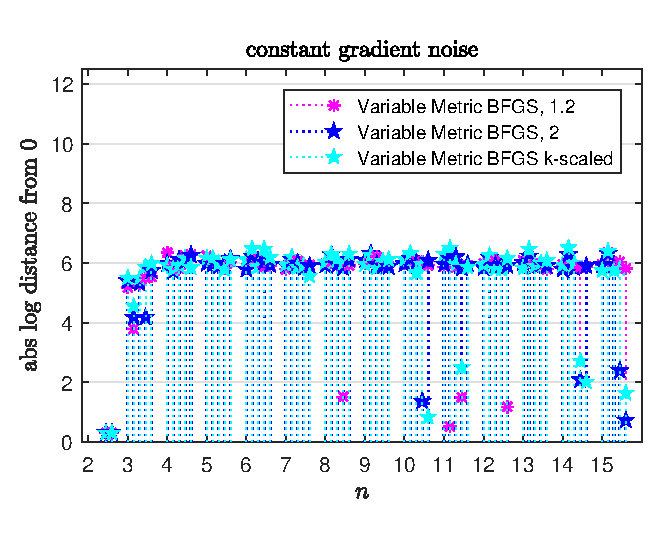
\includegraphics[width=\textwidth]{Pictures/Plots/constant_gradient_noise_comp.eps}%
	\end{subfigure}
	\begin{subfigure}{0.49\textwidth}
		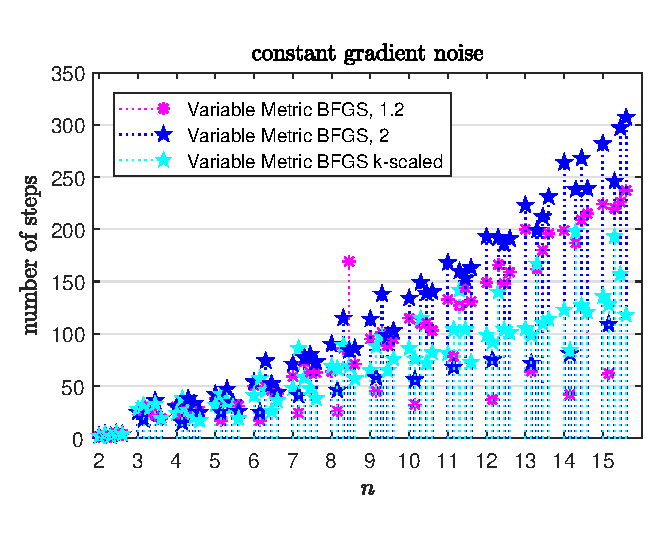
\includegraphics[width=\textwidth]{Pictures/Plots/steps_constant_gradient_noise_comp.eps}%
	\end{subfigure}
	\caption{Influence of the step size updating parameter \(\kappa_+ = 1.2\) and \(\kappa_+ =2 \) and performance of the hybrid method for constant gradient noise.}%
	\label{fig_const_grad_noise_comp}%
\end{figure}

\vspace{-1.5em}

\begin{figure}[H]
	\begin{subfigure}{0.49\textwidth}
		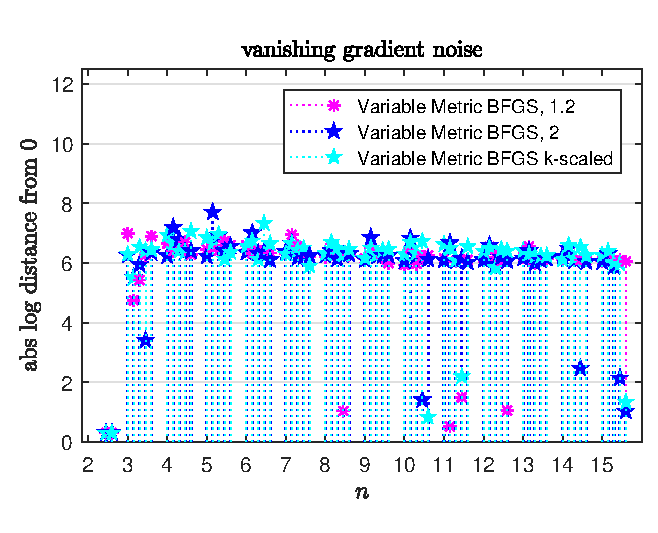
\includegraphics[width=\textwidth]{Pictures/Plots/vanishing_gradient_noise_comp.eps}%
	\end{subfigure}
	\begin{subfigure}{0.49\textwidth}
		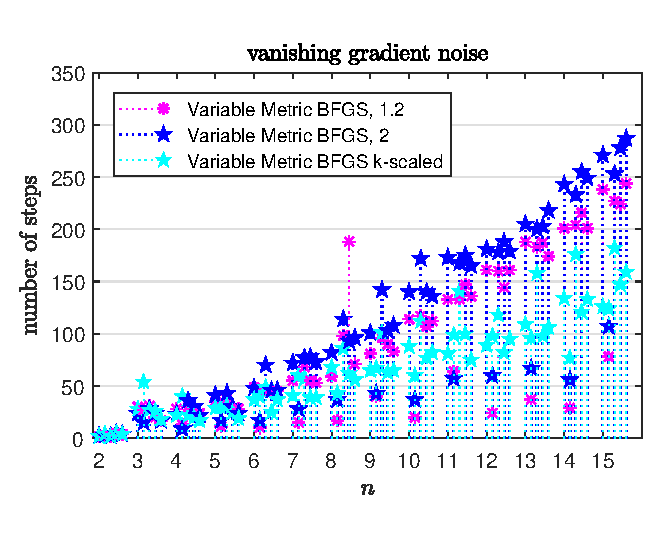
\includegraphics[width=\textwidth]{Pictures/Plots/steps_vanishing_gradient_noise_comp.eps}%
	\end{subfigure}
	\caption{Influence of the step size updating parameter \(\kappa_+ = 1.2\) and \(\kappa_+ =2 \) and performance of the hybrid method for vanishing gradient noise.}%
	\label{fig_van_grad_noise_comp}%
\end{figure}

\vspace{-1.5em}


%Following plots are in Noll part with \(\kappa_+ = 1.2, 2\) and in \(1/k\) part with \(\kappa_+ = 1.2\) for the large dimension
\begin{figure}[H]%
	\begin{subfigure}{0.49\textwidth}
		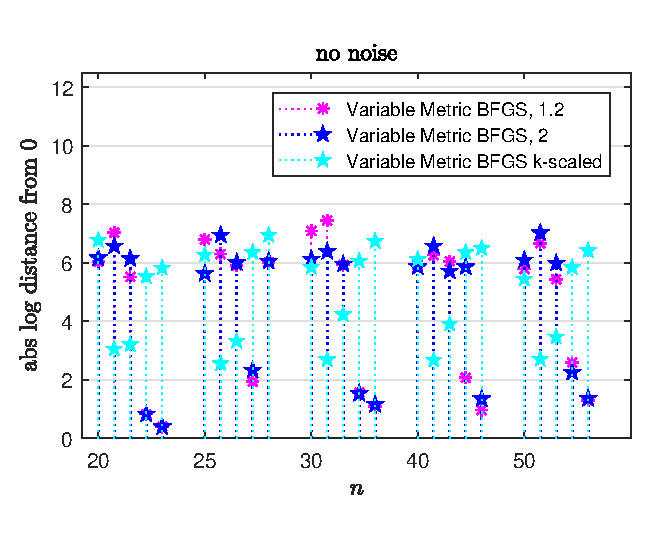
\includegraphics[width=\textwidth]{Pictures/Plots/no_noise_compb.eps}%
	\end{subfigure}
	\begin{subfigure}{0.49\textwidth}
		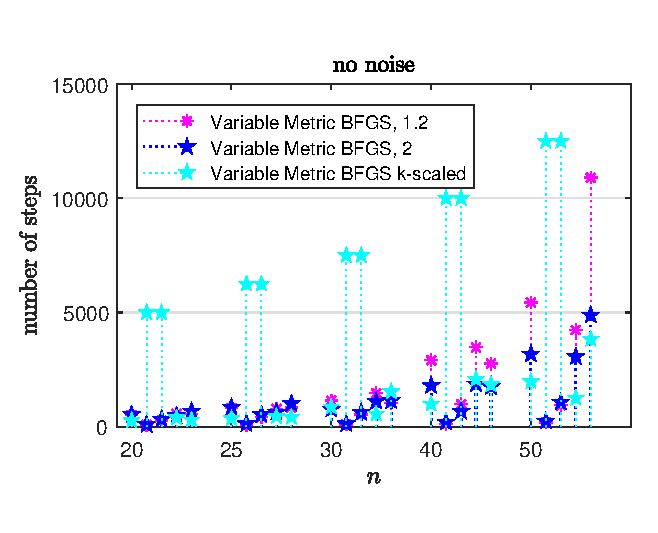
\includegraphics[width=\textwidth]{Pictures/Plots/steps_no_noise_compb.eps}%
	\end{subfigure}
	\label{fig_no_noise_comp_large}
	\caption{Influence of the step size updating parameter \(\kappa_+ = 1.2\) and \(\kappa_+ =2 \) and performance of the hybrid method for the exact case for higher \(x\)-dimensions. The reached accuracy is depicted on the left, the needed number of steps on the right.}
\end{figure}

\vspace{-1.5em}

\begin{figure}[H]
	\begin{subfigure}{0.49\textwidth}
		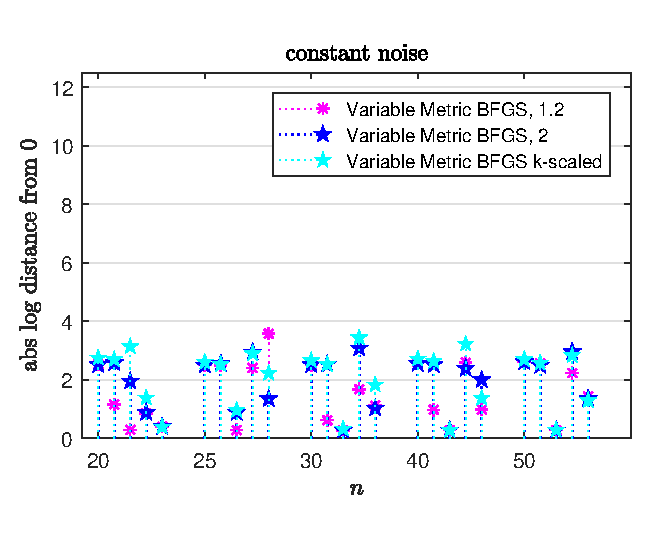
\includegraphics[width=\textwidth]{Pictures/Plots/constant_noise_compb.eps}%
	\end{subfigure}
	\begin{subfigure}{0.49\textwidth}
		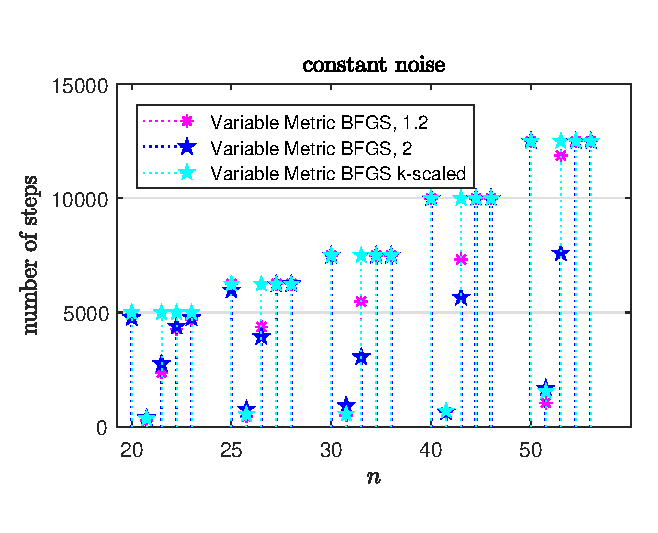
\includegraphics[width=\textwidth]{Pictures/Plots/steps_constant_noise_compb.eps}%
	\end{subfigure}
	\caption{Influence of the step size updating parameter \(\kappa_+ = 1.2\) and \(\kappa_+ =2 \) and performance of the hybrid method for constant noise.}%
	\label{fig_const_noise_comp_large}%
\end{figure}

\vspace{-1.5em}

\begin{figure}[H]
	\begin{subfigure}{0.49\textwidth}
		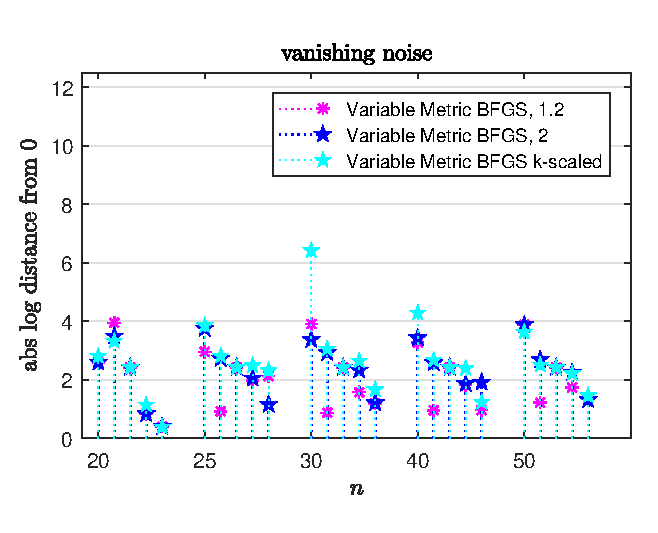
\includegraphics[width=\textwidth]{Pictures/Plots/vanishing_noise_compb.eps}%
	\end{subfigure}
	\begin{subfigure}{0.49\textwidth}
		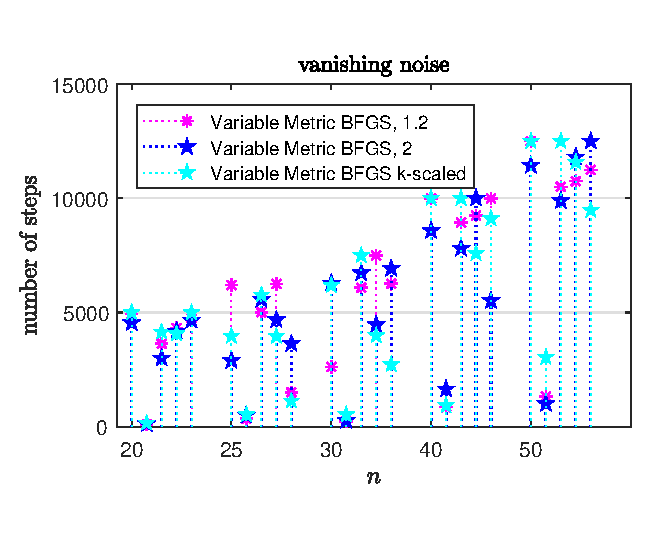
\includegraphics[width=\textwidth]{Pictures/Plots/steps_vanishing_noise_compb.eps}%
	\end{subfigure}
	\caption{Influence of the step size updating parameter \(\kappa_+ = 1.2\) and \(\kappa_+ =2 \) and performance of the hybrid method for vanishing noise.}%
	\label{fig_van_noise_comp_large}%
\end{figure}

\vspace{-1.5em}

\begin{figure}[H]
	\begin{subfigure}{0.49\textwidth}
		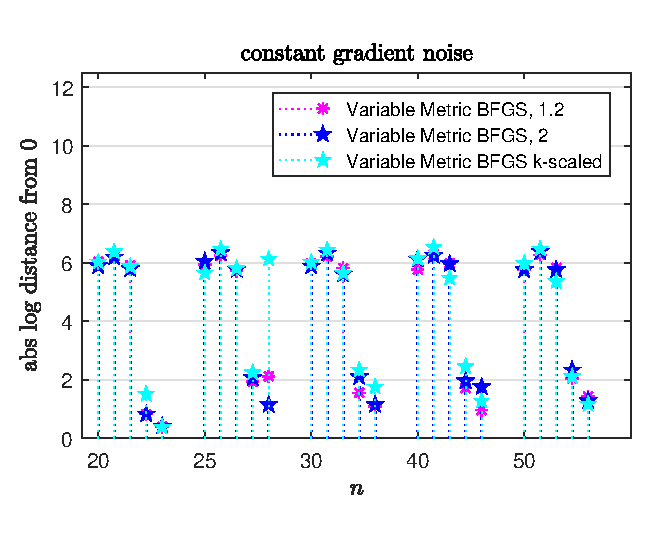
\includegraphics[width=\textwidth]{Pictures/Plots/constant_gradient_noise_compb.eps}%
	\end{subfigure}
	\begin{subfigure}{0.49\textwidth}
		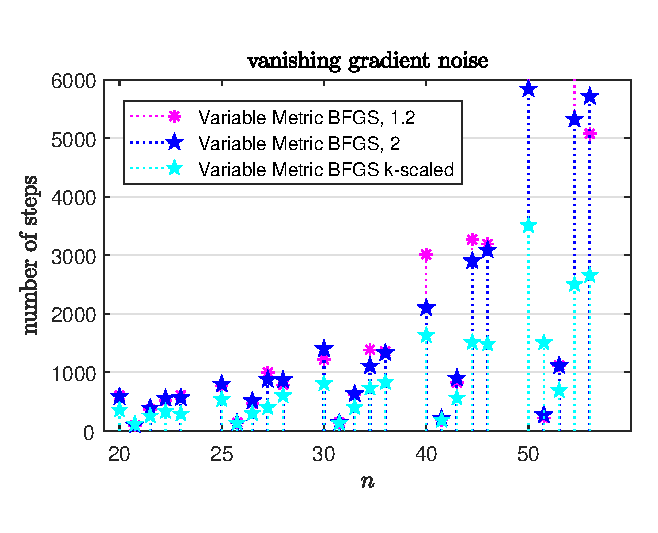
\includegraphics[width=\textwidth]{Pictures/Plots/steps_constant_gradient_noise_compb.eps}%
	\end{subfigure}
	\caption{Influence of the step size updating parameter \(\kappa_+ = 1.2\) and \(\kappa_+ =2 \) and performance of the hybrid method for constant gradient noise.}%
	\label{fig_const_grad_noise_comp_large_large}%
\end{figure}

\vspace{-1.5em}

\begin{figure}[H]
	\begin{subfigure}{0.49\textwidth}
		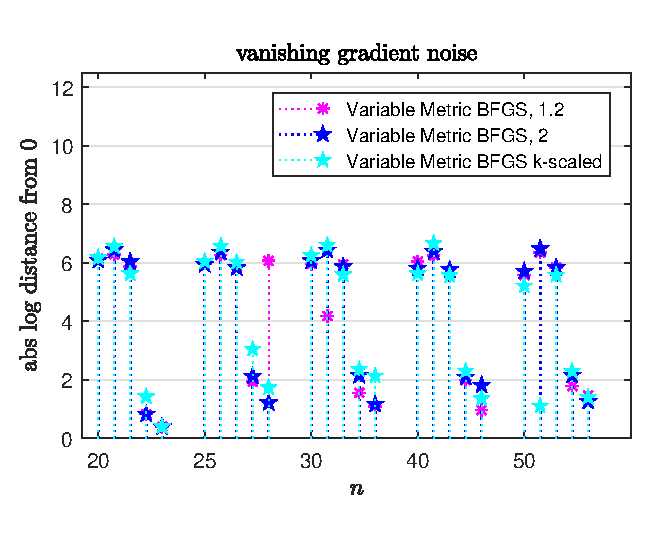
\includegraphics[width=\textwidth]{Pictures/Plots/vanishing_gradient_noise_compb.eps}%
	\end{subfigure}
	\begin{subfigure}{0.49\textwidth}
		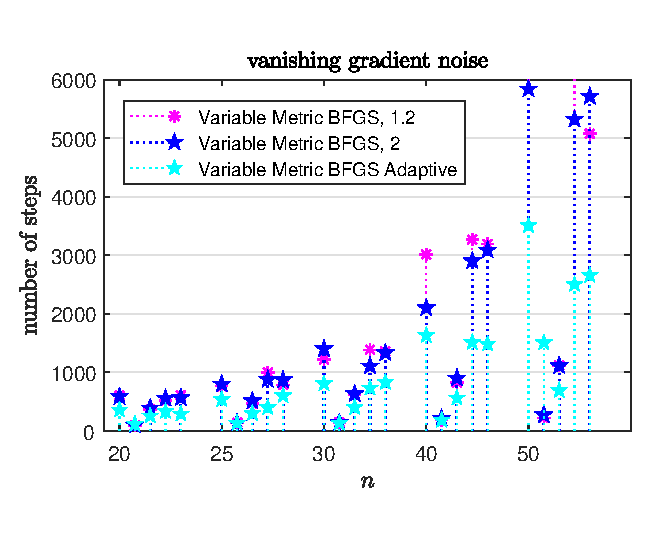
\includegraphics[width=\textwidth]{Pictures/Plots/steps_vanishing_gradient_noise_compb.eps}%
	\end{subfigure}
	\caption{Influence of the step size updating parameter \(\kappa_+ = 1.2\) and \(\kappa_+ =2 \) and performance of the hybrid method for vanishing gradient noise.}%
	\label{fig_van_grad_noise_comp_large}%
\end{figure}

